\cleartooddpage[\thispagestyle{empty}]
\newcommand{\Like}{L}
\newcommand{\LogLike}{\mathcal{L}}
\newcommand{\LogLikeMax}{\LogLike_{\textrm{max}}}
\newcommand{\xtrue}{\mathbf{x }}
\newcommand{\xdet }{\mathbf{x'}}
\newcommand{\ltrue}{\mathbf{l }}
\newcommand{\ldet }{\mathbf{l'}}
\newcommand{\btrue}{\mathbf{b }}
\newcommand{\bdet }{\mathbf{b'}}
\newcommand{\Etrue}{\mathbf{E }}
\newcommand{\Edet }{\mathbf{E'}}
\newcommand{\ttrue}{\mathbf{t }}
\newcommand{\tdet }{\mathbf{t'}}
\newcommand{\Aeff }{A_\textrm{eff }}
\newcommand{\Edisp}{E_\textrm{disp}}
\newcommand{\Mnull}{M_\textrm{null}}
\newcommand{\Malt }{M_\textrm{alt }}

\chapter{A Likelihood Search for Dark Matter}\label{chapter:analysis}

\section{Veritas Data}\label{veritasdata}
  The analysis in this thesis relies on three sets of VERITAS data.
  One set contains observations of the Crab Nebula, and another of the Galactic Center.
  A third set contains observations of a dark region \nicetilde\ang{5} away from the Galactic Center.
  This dark region is referred to as  Sgr A* Off, and is located at (l,b)=(\ang{357.3396}, \ang{3.9984}).
  Sgr A* Off is located a few degrees away to avoid the bright diffuse gamma-ray emission caused by the galactic plane.
  The Galactic Center and Sgr A* Off observation regions are shown in Figure~\ref{fig:gcfieldsofview}.
  To quantify the detector efficiency, observations are taken at \ang{0.5} or \ang{0.7} offsets from each observing target, in four different directions (wobbles) along right ascension/declination axes.

  \begin{figure}[!ht]
    \centering
    \includegraphics[width=0.85\textwidth]{images/skypointings/plot.pdf}
    \caption[VERITAS Galactic Center Pointings]{
      Fields of view for Galactic Center observations.
      Each circle marks the detection area of one telescope pointing.
      Green circles are Galactic Center observations, while dark blue circles are the Sgr A* Off observations used to construct the camera-background templates.
      The light blue band is the galactic plane.
    }
    \label{fig:gcfieldsofview}
  \end{figure}

  All three sets of data include observations from both the V5 and V6 epochs (see Section~\ref{sec:epochs}).
  All used data was taken from April 2010 to June 2016.
  The specific VERITAS data run numbers are listed in Appendix~\ref{app:runlists}.

  \begin{table}[!ht]
    \centering
    \caption{Hours of observations taken at each source/epoch combination.}
    \label{tab:observation_times}
    \begin{tabular}{|l|l|l|l|}
      \hline
      \textbf{Epoch} & \textbf{Crab Nebula} & \textbf{Sgr A*} & \textbf{Sgr A* Off} \\ \hline
      V5             & 3.3                  & 46.3            & 13.0                \\ \hline
      V6             & 5.5                  & 62.7            & 4.7                 \\ \hline
      % times calculated with $VERIPY/thesis/plots/obs_times.py
    \end{tabular}
  \end{table}


  \begin{figure}[!ht]
    \centering
    %\includegraphics[width=0.95\textwidth]{images/data_elevation_plots/plot.pdf}
    \includegraphics[width=0.95\textwidth]{images/elevation_hist/elevhist.pdf}
    \caption[VERITAS Data Elevation Exposure]{
      Camera center elevation for the three sets of data.
      The three peaks in the Sgr A* data are from the 4 wobble positions being at different elevations.
      The North wobble observations peak at elevation \nicetilde\ang{29.75}, East and West wobbles observations at \nicetilde\ang{29.25}, and South wobble observations at \nicetilde\ang{28.75}.
    }
    \label{fig:datapointingelevations}
  \end{figure}

  There are comparativly fewer Sgr A* Off observations because this source is only used for background estimation, and telescope time is in high demand.
  There are also fewer Crab Nebula observations, as the majority of its data is taken at higher elevations, where the telescope has increased sensitivity to lower energies.
  
  For all of these observations, quality cuts were applied.
  This includes monitoring the telescope hardware and cloud ceiling in the field of view.
  Two far-infrared Pyropemeters are used to measure the cloud ceiling height, by measuring the temperature of the sky.
  With the pyrometer, clouds are significantly warmer (\nicetilde\ang{50} C) than clear sky.
  Low-quality segments of data, where there are large (>20\%) and/or rapid (<=\SI{30}{s}) changes in the L3 trigger rate or cloud ceiling height, are removed from the analysis~\cite{bird_weather}.
  % see Bird 2015 thesis pg 55

  Because each VERITAS epoch has a different hardware configuration, they also each have their own separate set of effective areas, point spread functions, energy migration matricies, and camera background models.
  In addition, specific IRFs were calculated for additional data dimensions, including the frequency of night sky background photons in the camera, the telescope elevation, the event energy, and each event's distance from the camera center.
  
  After this data is collected, it is used in a likelihood analysis, detailed in the next section.

\section{Likelihood Ratio Test}\label{sec:likeratio}
  A likelihood ratio test determines which of two model groups is a statistically better fit to a set of data.
  It is performed by calculating, for a group of events, the likelihood of detecting that group of events for each of two model groups.
  Once the likelhood is calculated, then the parameters of the model are varied until the maximum likelihood is found for each model.
  These two maximum likelihoods can then be used to calculate the test statistic (TS), which determines which model is statistically favored, and to what degree it is favored.
  
  \subsection{Likelihood Calculation}
  At its heart, a likelihood is a product of probabilities.
  With two events, the likelihood is $(\textrm{probability that event 1 happens})\times(\textrm{probability that event 2 happens})$.
  In a counting experiment like VERITAS, the likelihood $\Like$ is determined via poissonian statistics, shown in Equation~~\ref{eqn:simple_like}.
  In this equation, $n$ is the number of observed events, and $m$ is the average number of events predicted by a model group.
  
  \begin{equation}\label{eqn:simple_like}
    \Like = \frac{e^{-m} m^n}{n!}
  \end{equation}
  
  For increased statistical power, the VERITAS data can be split into bins in energy, galactic $l$ and $b$, and time.
  When combining multiple bins arbitrarily ordered by index $j$, each bin's likelihood is multiplied together as in Equation~\ref{eqn:simple_like_2}.
  These events could be binned in dimensions of sky position, energy, time, or other event parameters, or any combination of these parameters.
  Future likelihood calculations may also include shower core position on the ground, or distance to the shower, or other observables.
  
  \begin{equation}\label{eqn:simple_like_2}
    \Like = \prod_j \frac{ e^{-m_j} \; m_{j}^{n_j}}{n_{j}!}
  \end{equation}

  Equation~\ref{eqn:simple_like_2} is a general formula for calculating a binned likelihood of poissonian events.
  As events are grouped by bins, some information is lost, which generally results in a less powerful ratio test.
  The result in Equation~\ref{eqn:simple_like_2} can be expanded into an unbinned likelihood through the following derivation.
  First, Equation~\ref{eqn:simple_like_2} can be rearranged:
  
  \begin{equation}\label{eqn:simple_like_3}
    \Like = \prod_j e^{-m_j} \prod_j \frac{m_j^{n_j}}{n_{j}!}
  \end{equation}
    
  \begin{equation}\label{eqn:simple_like_4}
    \Like = e^{- \sum_j m_j} \prod_j \frac{m_j^{n_j}}{n_{j}!}
  \end{equation}
  
  Then, the size of each bin can be shrunk until there are only 1 or 0 events in each bin.
  For empty bins (where $n=0$), the product in Equation~\ref{eqn:simple_like_4} becomes
  
  \begin{equation}\label{eqn:simple_like_4a}
    n=0 \rightarrow \frac{m_j^{n_j}}{n_j!} = \frac{m_j^{0}}{0!} = \frac{1}{1} = 1 .
  \end{equation}

  For bins with 1 event, the product in Equation~\ref{eqn:simple_like_4} becomes

  \begin{equation}\label{eqn:simple_like_4b}
    n=1 \rightarrow \frac{m_j^{n_j}}{n_j!} = \frac{m_j^1}{1!} = \frac{m_j}{1} = m_j = m_i ,
  \end{equation}

  where $i$ is the $i^{\textrm{th}}$ event, and $m_i$ is the number of predicted events at event $i$'s sky position, energy, and time.
  In this derivation, $m_j$ converts to $m_i$, because all the $n=0$ bins are now 1 and can be ignored, so a loop over the $j$ bins becomes a loop over the $i$ events.
  Then Equation~\ref{eqn:simple_like_4} becomes Equation~\ref{eqn:simple_like_5}.
  
  \begin{equation}\label{eqn:simple_like_5}
    \Like = e^{- \sum_j m_j} \prod_i m_i
  \end{equation}
  
  In Equation~\ref{eqn:simple_like_5}, $\prod_i m_i$ encodes the data events, while $\sum_j$ encodes the model information.
  When calculating $\Like$, certain computational problems can arise.
  Calculating the product of many small probabilities can result in extremely small numbers, beyond the binary storage limit of common variable types.
  Calculating derivatives of some of these numbers is computationally expensive, so to solve these two problems, the log-likelihood $\LogLike$ is instead calculated.
  
  \begin{equation}\label{eqn:simple_like_6}
    \LogLike = \textrm{log} \left ( \Like \right ) 
  \end{equation}
  
  This is possible because both $\Like$ and $\LogLike$ are both strictly increasing functions, so the maximum of both will be at the same position in the parameter space.
  The log-likelihood for a group of bins is then:
  
  \begin{equation}\label{eqn:simple_like_7}
    \LogLike = \textrm{log} \left ( e^{- \sum_j m_j} \prod_i m_i \right ) = - \sum_j m_j + \sum_i \textrm{log} \left ( m_i \right )
  \end{equation}
  
  When the bin size is infinitely small, $m_i$ becomes $P_i$, the value of the probability density function (of all models combined) at the position of the event, as in Equation~\ref{eqn:simple_like_8}.
  
  \begin{equation}\label{eqn:simple_like_8}
    \LogLike = \textrm{log} \left ( e^{- \sum_j m_j} \prod_i m_i \right ) = - \sum_j m_j + \sum_i \textrm{log} \left ( P_i \right )
  \end{equation}
  
  The unbinned Equation~\ref{eqn:simple_like_8} shows how the log-likelihood is calculated in this analysis.
  The $\sum_{j} m_{j}$ term can be interpreted as the total number of events predicted by all models, sometimes referred to as $N_{pred}$.
  Please note however, that while a binned likelihood calculation scales with the number of bins (and some lost information), the unbinned likelihood calculation scales with the number of events, which can lead to large likelihood maximization times (see later in this section).
  
  \subsection{Models}\label{sec:model_irf_folding}
  
  Models are used in a likelihood analysis to predict the number of events that a particular source deposits into a particular bin.
  In a likelihood analysis, each source of events gets its own model.
  Each model is described by a function $M$, and different sources will have different $M$ functions.
  The function $M$ has dimensional units of $\frac{\textrm{counts}}{\textrm{energy}\times\textrm{solid angle}\times\textrm{area}\times\textrm{time}}$.
  This function can be integrated over the energy, sky, and time region covered by a bin to calcuate the number of events predicted in that bin, as shown by Equation~\ref{eqn:model_int}.
  
  \begin{equation}\label{eqn:model_int}
    m_{i \, \textrm{or} \, j} = \int_{t\,\textrm{bin}} \int_{E\,\textrm{bin}} \int_{b\,\textrm{bin}} \int_{l\,\textrm{bin}} M(l,b,E,t)\; dl \; db \; dE \; dt
  \end{equation}
  
  In this equation, $l$ and $b$ are sky coordinates, $E$ is energy, and $t$ is time.
  The basic models used in this analysis can be broken apart into their spatial, spectral, and temporal components, as in Equation~\ref{eqn:modelparts}.

  \begin{equation}\label{eqn:modelparts}
    M(l,b,E,t) = M_s(l,b,E,t) \; \; M_e(l,b,E,t) \; \; M_t(l,b,E,t)
  \end{equation}
  
  For this thesis, the sources being modeled are either constant in flux, or in equilibrium, so time-dependent effects are ignored by setting $M_{t}(l,b,E,t) = 1$.

  For a basic point source, the spatial model function $M_s$ is shown in Equation~\ref{eqn:pntsrc_Ms}.

  \begin{equation}\label{eqn:pntsrc_Ms}
    M_{s,\textrm{point}}(l,b,E,t) = \lim_{a\to\infty} \frac{1}{ \abs{a} \sqrt{\pi} } e^{ - \left ( \sqrt{ (l-l_o)^2 + (b-b_o)^2 }/a \right )^2 }
  \end{equation}
  
  In this equation, $l_o$ and $b_o$ specify the position of the point source in Galactic sky coordinates, which can be model parameters.
  More complex $M_s$ functions may also have the spatial structure depend on energy $E$ or time $t$, or may take on other spatial shapes like an ellipse or a radially-symmetric profile.
  The energy spectrum can be similarly modeled by a basic power law.
  This basic power law is defined by the model function $M_e$, and is shown in Equation~\ref{eqn:powerlaw_Me}.
  
  \begin{equation}\label{eqn:powerlaw_Me}
    M_{e,\textrm{powerlaw}}(l,b,E,t) = N_o \left ( \frac{E}{E_o} \right )^{-\gamma}
  \end{equation}

  In this equation, $N_o$ is the flux normalization, $E_o$ is the pivot energy, and $\gamma$ is the spectral index, which can all be model parameters.

  
  \subsection{Instrument Response Function Folding}\label{subsec:folding}
  The average number of counts predicted by a model is calculated by integrating over the entire energy, sky, and time regions in the analysis.
  Because the reconstruction method is not perfect, all events from the astrophysical models are diffused according to the PSF and Energy Dispersion.
  Another way of understanding this is that if a source is located in some sky bin $j$, events from that source can be reconstructed in neighboring bins $j+1$ and $j-1$, increasing the predicted number of events in those bins and decreasing the number of events in bin $j$, as determined by the PSF.
  This dispersion is illustrated in Figure~\ref{fig:responsedispersion}.
  Similarly, energy dispersion will diffuse events out among neighboring energy bins as well.
  
  \begin{figure}[!t]
    \centering
    \includegraphics[width=0.85\textwidth]{images/responsefunction/responsefunction.pdf}
    \caption[Response Function Dispersion]
    {
      Left: Events from a source at the green arrow detected by a 'perfect' detector, with bins in true coordinates.
      Right: The same events detected by a 'real-world' detector, with bins in reconstructed coordinates.
    }
    \label{fig:responsedispersion}
  \end{figure}
  
  This leads to the need to define two distinct coordinate systems, $\xtrue$ and $\xdet$.
  $\xtrue$ is a coordinate in true space (galactic $\ltrue$ and $\btrue$, energy $\Etrue$, and time $\ttrue$) space, \textit{before} folding is applied.
  Alternatively, $\xdet$ is the coordinate in reconstructed detector space ($\ldet$ and $\bdet$, $\Edet$, and $\tdet$), \textit{after} folding is applied.
  Another way this can be thought of is that $\xtrue$ is the physical coordinates for events \textit{before} they reach Earth's atmosphere, and $\xdet$ is \textit{after} the events have been reconstructed.
  Equation~\ref{eqn:folding} shows this integration.
  
  \begin{equation}\label{eqn:folding}
    P_i \left( \xdet \right ) = \int_\xtrue R \left ( \xdet, \xtrue \right ) * M \left ( \xtrue \right ) d\xtrue
  \end{equation}
  
  Here, $P_i \left( \xdet \right )$ is the probability of detecting an event at detector coordinates $\xdet = \left ( \ldet, \bdet, \Edet, \tdet \right )$.
  The integration $\int_\xtrue$ takes place over the entire true space, time, and energy regions being studied.
  The function $M\left ( \xtrue \right )$ is the number of counts predicted by the astrophysical models at coordinate $\xtrue$, and $R \left ( \xdet, \xtrue \right )$ is the dispersion at $\xdet$ due to $\xtrue$.
  The function $R$ (the instrument Response function) incorporates the Effective Area, PSF, and Energy Dispersion information as shown in Equation~\ref{eqn:foldingR}, and is discussed further in Sections \ref{subsec:effarea}, \ref{subsec:psf}, and \ref{subsec:edisp}.
  
  \begin{equation}\label{eqn:foldingR}
    R(\xdet,\xtrue) = \Aeff(\xtrue) * PSF(\xdet,\xtrue) * \Edisp(\Edet,\xtrue)
  \end{equation}
  
  In Equation~\ref{eqn:foldingR}, functions $\Aeff$, $PSF$, and $\Edisp$ are all interpolated from tables of stored values, which are derived from simulations.

  The Crab Nebula point source in Section~\ref{sec:crab_analysis}, the Galactic Center point source in Section~\ref{subsec:gcpointsrc}, and the dark matter halo model in Section~\ref{subsec:dmhalomodel} all have this folding applied to the number of events they predict.
  An important distinction is that this folding is only applied to these astrophysical models, and not to the camera background models.
  This is because the background models are created with data from actual observations, which have the folding already applied, and thus are already in $\xdet$ space.
  
  \subsection{Combining Models into Hypotheses}\label{subsec:hypotheses}
  
  When calculating the likelihood of a bin in Equation~\ref{eqn:simple_like}, the predicted number of counts in a bin may come from a combination of sources.
  Some fraction may come from a background model, another fraction from a specific source model, and still others from other models.
  So in order to account for these multiple models, their predicted counts in a bin must be summed first, as in Equation~\ref{eqn:combinemodels}, before being used in Equation~\ref{eqn:simple_like_8}.
  
  \begin{equation}\label{eqn:combinemodels}
    m_{i\,\textrm{or}\,j} = \sum_k m_k(i\,\textrm{or}\,j)
  \end{equation}

  In Equation~\ref{eqn:combinemodels}, index $k$ loops over the various models that contribute events to a particular bin.
  The factor $m_k$ represents the number of counts predicted by model $k$, at the position of event $i$ or bin $j$.
  
  In order to calculate a test statistic, the models must be grouped into two sets, called hypotheses.
  For a basic analysis, the null hypothesis consists of all models, except the one in particular being searched for, called here $\Mnull$.
  The second hypothesis, called the alternate hypothesis, consists of all the models in the null hypothesis, plus the model being searched for, called here $\Malt$.
  Each observation would get its own camera background model, and then any additional astrophysical models are added separately.
  For example, if one has three observations of the Crab Nebula, this would mean there are three camera background models, plus a point source model for the Crab Nebula.
  The null hypothesis would be just the camera background models, while the alternate hypothesis would be the camera backgrounds plus the Crab Nebula model.
  Once these two hypotheses for an analysis are assembled, then their maximum likelihood can be searched for.
  
  \subsection{Likelihood Maximization}\label{subsec:likemax}
  This maximum likelihood is found by iteratively changing the parameters of a hypothesis's component models in directions that increase the likelihood.
  For example, take the alternate hypothesis used in Section~\ref{subsec:hypotheses}, with three camera background models and one Crab Nebula point source.
  Each camera background model has a base template multiplied by a power law.
  Each power law has two parameters, a normalization and a spectral index, so the background camera models have the parameters $N_1$, $N_2$, $N_3$, $\gamma_1$, $\gamma_2$, and $\gamma_3$.
  The Crab Nebula point source power law also has normalization and spectral index parameters $N_c$ and $\gamma_c$.
  The Crab Nebula model also has location parameters $l_c$ and $b_c$, but since these are fixed in this example (and thesis), the likelihood maximization can't vary them.
  Therefore this alternate hypothesis would have 8 free parameters, $N_1$, $N_2$, $N_3$, $N_c$, $\gamma_1$, $\gamma_2$, $\gamma_3$, and $\gamma_c$.
  For calculating the test statistic for the presence of the Crab Nebula, the null hypothesis is just the camera background models, with 6 free parameters $N_1$, $N_2$, $N_3$, $\gamma_1$, $\gamma_2$, and $\gamma_3$.
  
  When finding the maximum likelihood for each hypothesis, these free parameters are incrementally varied, and the likelihood is recalculated.
  This procedure is repeated until a maximum likelihood is reached.
  While there are many maximization algorithms, this analysis uses the Levenberg-Marquardt method~\cite{marquardt1963algorithm}.
  Once the maximum likelihood is calculated for both hypotheses, then the test statistic can be calculated.
  
  \subsection{Test Statistic Calculation}
  
  In order to search for the presence of a source, the test statistic (TS) determines how favorable the alternate hypothesis is compared to the null hypothesis.
  Once the maximum likelihood $\LogLike_{\textrm{max}}$ is found for these two hypotheses, the TS can be calculated with Equation~\ref{eqn:tscalc}.
  
  \begin{equation}\label{eqn:tscalc}
    \textrm{TS} = - 2 \; \textrm{log} \left (  \frac{ \LogLikeMax( \Mnull ) }{ \LogLikeMax( \Malt ) } \right )
  \end{equation}
  
  With Wilk's theorem~\cite{wilks1938}, the events can be repeatedly simulated using the null hypothesis probability density function.
  For each simulation, a TS can be calculated.
  After many simulations, the resulting TS's will form a $\chi^2$ distribution with $n$ degrees of freedom, where $n$ is the difference in number of free parameters between the two hypotheses.
  From this simulated TS distribution, an actual TS can be converted into a p-value.
  In situations where there is only one or two degrees of freedom, the significance of a specific model can be calculated as $\sqrt{\textrm{TS}}$.
  Due to time constraints, the p-value of this test statistic was not calculated.
  % http://pulsar.sternwarte.uni-erlangen.de/black-hole/2ndschool/talks/likelihood_1.pdf
  

\section{Background Models}\label{sec:bkgmodels}
  The background models predict the amount of background counts produced by a sky without gamma rays.
  This is used to model the probability density function of the background (primarily proton) events, which are several orders of magnitude more populous than the gamma rays.
  Background models are produced by binning observation sources with weak or no gamma-ray emission.
  For this low-elevation analysis the observations of the dark region Sgr A* Off, described in Section~\ref{veritasdata}, were used to build these backgrounds.
  These dark region events were then binned into background models, using the method described in Section~\ref{background_production}.
  To account for the difference between the V5 and V6 observatory configurations, the background observations are divided up based on their VERITAS hardware epoch, producing a unique background template for each epoch.
  These background templates only depend on the radial distance from the camera center and the event energy.
  These background templates are used in both the Crab Nebula analysis and the Galactic Center analysis.
  This can be done because the templates are made from Sgr A* Off, which has no sources of gamma-rays, so only the detectable events are due to background protons.

\section{Crab Nebula Likelihood Analysis}\label{sec:crab_analysis}
  To verify that the likelihood method is physically correct, the Crab Nebula was analyzed first, before any dark matter analysis was performed.
  As the Crab Nebula is the brightest gamma ray emitter in the sky, it has been observed extensively by VERITAS and other gamma ray telescopes.
  After searching for low-elevation Crab Nebula observations, a total of 17.1 hours of data were selected from the VERITAS data archives.
  Since the Galactic Center only rises to around \ang{30} elevation, elevation effects would also need to be searched for.
  To uncover any low-elevation effects, time cuts were applied to this data to restrict the telescope pointing elevations to \SIrange{27.5}{32.5}{\degree}, similar to the Galactic Center data later on (see Figure~\ref{fig:datapointingelevations}).
  This resulted in \SI{3.3}{hours} of V5 and \SI{5.5}{hours} of V6 epoch data (see Table \ref{tab:observation_times}).
    
  \begin{figure}[!t]
    \centering
    %\includegraphics[width=0.85\textwidth]{images/test_crab_analysis/plot_elev27_5_32_5deg_4_70TeV_wobbleall_Epochall_skymap.pdf}
    \includegraphics[width=0.85\textwidth]{images/test_crab_analysis/plot_elev27_5_32_5deg_4_70TeV_nfits165_mapcounts.pdf}
    \caption[Crab Nebula Counts Skymap]
    {
      Skymap of event positions, ($\ldet$,$\bdet$).
      No corrections are made for observing time or effective area.
    }
    \label{fig:crab_skymap}
  \end{figure}
  
  The Crab Nebula is modeled by a point source with the simple power law spectrum in Equation~\ref{eqn:crab_model}.
  These spatial and spectral shapes are both discussed in Section~\ref{subsec:likemax}.

  \begin{equation}\label{eqn:crab_model}
    M(\xtrue) = M_{s,\textrm{powerlaw}}(\xtrue) * M_{e,\textrm{point}}(\xtrue) = N_o \left ( \frac{\Etrue}{E_o} \right )^{-\gamma} * \lim_{a\to\infty} \frac{1}{ \abs{a} \sqrt{\pi} } e^{ - \left ( \sqrt{ (\ltrue-l_c)^2 + (\btrue-b_c)^2 }/a \right )^2 }
  \end{equation}

  The sky position of the point source is fixed to the Crab Nebula, at

  $$(l_c,b_c) = (\ang{184.557600},\ang{-5.784180}) \;\;.$$

  The pivot energy $E_o$ of its spectrum is fixed at \SI{16.73}{\TeV{}}, while the normalization $N_o$ and the spectral index $\gamma$ are free to vary during the likelihood optimization.
  Only events between \SIrange{4}{70}{\TeV{}} are used in this test analysis.
  At an elevation of \ang{25}, the reconstruction method is able to reconstruct events as low as \SI{1.5}{\TeV{}}.
  Below \SI{4}{\TeV{}} however, the camera sensitivity starts to decrease in a poorly understood way, and IRFs in this region may not be accurate.
  Part of this decrease is explored in Section~\ref{subsec:bkgstructure} (see Figures \ref{fig:bkgvsel_crab} and \ref{fig:bkgvsel_sgra}), but accounting for this requires an unfeasibly large set of simulations.
  At energies above \SI{200}{\TeV{}}, simulations become too computationally expensive when attempting to calculate IRFs.
  In order to ensure there are enough simulations to properly populate the high-energy end of the IRFs, the analysis is limited to a maximum event energy of \SI{70}{\TeV{}}.
    
  % values from nkelhos@warp-zeuthen.desy.de:/afs/ifh.de/group/cta/scratch/nkelhos/dm_halo_testing/veripy/thesis/analysis/crab_test/logs/statistics.txt
  After fitting all model parameters to the events from \SIrange{4}{70}{\TeV{}}, the best fit power law values are $ N_o = \left(3.90\pm0.71\right)*10^{-20} \frac{\textrm{photons}}{\textrm{cm}^{2} \; \textrm{s} \; \textrm{MeV} } $, $ \gamma = 2.31 \pm 0.17 $, with a test statistic of 408.8, corresponding to \nicetilde{}\SI{20.2}{$\sigma$}.
  As the alternate Crab Nebula hypothesis has 110 free parameters, and the no-Crab-Nebula (null) hypothesis has 108 free parameters, the test statistic has $ 110 - 108 = 2 $ degrees of freedom.
  
  \begin{figure}[!t]
    \centering
    %\includegraphics[width=0.95\textwidth]{images/test_crab_analysis/plot_elev27_5_32_5deg_4_70TeV_wobbleall_Epochall.pdf}
    %\includegraphics[width=0.95\textwidth]{images/test_crab_analysis/plot_elev27_5_32_5deg_4_70TeV_spectra.pdf}
    \includegraphics[width=0.95\textwidth]{images/test_crab_analysis/plot_elev27_5_32_5deg_4_70TeV_nfits165_spectra.pdf}
    \caption[Crab Nebula Spectra]
    {
      Crab Nebula spectra from various analyses and observatories.
      The solid red line is the best-fit spectra from the CTOOLS analysis described in this chapter, using only events from \SIrange{4}{70}{\TeV{}}.
      The inner red envelope is the statistical fitting error on the solid red line.
      The outer red envelope is the combined statistical+systematic error.
      The dark blue line is the standard VERITAS Eventdisplay spectrum using the same set of observations.
      The dark blue datapoints are flux points for specific energy bins, from Eventdisplay.
      Light blue is a Crab Nebula spectrum from HESS~\cite{hess2006crab}.
      Purple is a previously published spectrum from VERITAS~\cite{veritas2015crab}.
      Orange is a spectrum from MAGIC~\cite{magic2015crab}.
    }
    \label{fig:crab_test_spectra}
  \end{figure}
    
  \begin{table}[!t]
    \centering
    \begin{tabular}{|r|c|c|c|c|c|}
      \hline
      \textbf{Analysis} & \textbf{Min}    & \textbf{Max}    & \textbf{FOV} & \textbf{PSF} & \textbf{$\sigma$} \\
      \textbf{Method}   & \textbf{Energy} & \textbf{Energy} &  \#          & \#           &                   \\
                        & TeV             & TeV             &  Events      & Events       &                   \\
      \hline 
      On/Off Region & 3.16 & 79.4 & 11197 & 145 & 21.3 \\
      Likelihood    & 4.00 & 70.0 & 9319  & 120 & 20.2 \\
      \hline 
    \end{tabular}
    \caption[Analysis Comparison]{
      Comparison between the two different Crab Nebula analyses, using the On/Off regions in Eventdisplay, and the Likelihood analysis in ctools.
    }
    \label{tab:crab_statistics}
  \end{table}

  In the standard VERITAS Eventdisplay analysis, the Crab Nebula is found to have a point source significance of \SI{21.3}{$\sigma$}, shown in Table~\ref{tab:crab_statistics}.
  However, the energy range of this Eventdisplay analysis was from \SIrange{3.16}{79.4}{\TeV{}}, which contained a total of 11197 events in the field of view.
  The likelihood analysis was from \SIrange{4}{70}{\TeV{}}, containing only 9319 events, \nicetilde17\% fewer events.
  This ratio persisted when the events were limited to within \ang{0.18} of the Crab Nebula, the approximate radius of the PSF at \SI{10}{\TeV{}} (145 vs 120 events).
  Thus, with \nicetilde17\% fewer events, the likelihood test detects the Crab Nebula at the same significance level, implying this likelihood method is more sensitive than the standard analysis alone.
  % event display: 3.16 TeV to 79.4 TeV
  % ctools       : 4    TeV to 70   TeV
  % from nkelhos@warp-zeuthen.desy.de:~/dm_halo_testing/veripy/thesis/analysis/crab_test/energy_range_event_count_difference.py
  In Figure~\ref{fig:crab_test_spectra}, the fitted Crab Nebula spectra is shown, along with literature results from earlier VERITAS, HESS, and MAGIC observations of the Crab Nebula.
  
  \begin{figure}[p]
    \centering
    \includegraphics[width=0.85\textwidth]{images/test_crab_analysis/plot_elev27_5_32_5deg_4_70TeV_nfits165_profiledata_spatiall_json.pdf}
    \llap{
      \makebox[13cm][l]{ % x position
        \raisebox{5.2cm}{     % y position
          {
            \setlength{\fboxsep}{0pt}
            \setlength{\fboxrule}{1pt}
            \fbox{
              \includegraphics[height=4cm]{images/test_crab_analysis/plot_elev27_5_32_5deg_4_70TeV_nfits165_profl_skymap_rasterized.pdf}
            }
          }
        }
      }
    }
    \caption[Crab Nebula Profile along Galactic $l$]
    {
      The top plot shows the number of counts along a \ang{0.15}-wide-slice the Crab Nebula, along the galactic $l$ axis ($\ldet$ coordinate space).
      Blue points are the number of observed counts, with poissonian error bars~\cite{poissonfrequentistinterval}.
      The green histogram bars are the number of counts predicted by all models.
      Yellow histogram bars are the number of counts predicted by only the camera-background models.
      The red arrow indicates the position of the Crab Nebula.
      The bottom plot shows the $\mathrm{All\,Models}/\mathrm{Data}$ residual as green points, with the same blue poissonian error bars from the top plot.
      The inset plot shows the counts map from Figure~\ref{fig:crab_skymap}, with blue squares showing the profile bin locations.
    }
    \label{fig:crab_profile_l}
  \end{figure}

  \begin{figure}[p]
    \centering
    \includegraphics[width=0.85\textwidth]{images/test_crab_analysis/plot_elev27_5_32_5deg_4_70TeV_nfits165_profiledata_spatialb_json.pdf}
    \llap{
      \makebox[13cm][l]{ % x position
        \raisebox{5.2cm}{  % y position
          {
            \setlength{\fboxsep}{0pt}
            \setlength{\fboxrule}{1pt}
            \fbox{
              \includegraphics[height=4cm]{images/test_crab_analysis/plot_elev27_5_32_5deg_4_70TeV_nfits165_profb_skymap_rasterized.pdf}
            }
          }
        }
      }
    }
    \caption[Crab Nebula Profile along Galactic $b$]
    {
      The top plot shows the number of counts along a \ang{0.15}-wide-slice through the Crab Nebula along the galactic $b$ axis ($\bdet$ coordinate space).
      Blue points are the number of observed counts, with poissonian error bars~\cite{poissonfrequentistinterval}.
      The green histogram bars are the number of counts predicted by all models.
      Yellow histogram bars are the number of counts predicted by only the camera-background models.
      The red arrow indicates the position of the Crab Nebula.
      The bottom plot shows the $\mathrm{All\,Models}/\mathrm{Data}$ residual as green points, with the same blue poissonian error bars from the top plot.
      The inset plot shows the counts map from Figure~\ref{fig:crab_skymap}, with blue squares showing the profile bin locations.
    }
    \label{fig:crab_profile_b}
  \end{figure}
    
  \begin{figure}[p]
    \centering
    \includegraphics[width=0.85\textwidth]{images/test_crab_analysis/plot_elev27_5_32_5deg_4_70TeV_nfits165_profiledata_spatiallalt_json.pdf}
    \llap{
      \makebox[13.2cm][l]{ % x position
        \raisebox{6.8cm}{  % y position
          {
            \setlength{\fboxsep}{0pt}
            \setlength{\fboxrule}{1pt}
            \fbox{
              \includegraphics[height=2.4cm]{images/test_crab_analysis/plot_elev27_5_32_5deg_4_70TeV_nfits165_profa_skymap_rasterized.pdf}
            }
          }
        }
      }
    }
    \caption[Crab Nebula Profile along Galactic $l$ Off Source]
    {
      The top plot shows the number of counts along a \ang{0.15}-wide-slice along the galactic $l$ axis ($\ldet$ coordinate space).
      This slice doesn't go through the Crab Nebula, but instead \ang{1} higher in galactic $b$.
      As this doesn't include the Crab Nebula, this plot primarily demonstrates the camera background modeling.
      Blue points are the number of observed counts, with poissonian error bars~\cite{poissonfrequentistinterval}.
      The green histogram bars are the number of counts predicted by all models.
      The red arrow indicates the position of the Crab Nebula.
      As the Crab Nebula doesn't contribute any events \ang{1} to the North, the green histogram bars are identical (and behind) the yellow histogram bars.
      Yellow histogram bars are the number of counts predicted by only the camera-background models.
      The bottom plot shows the $\mathrm{All\,Models}/\mathrm{Data}$ residual as green points, with the same blue poissonian error bars from the top plot.
      The inset plot shows the counts map from Figure~\ref{fig:crab_skymap}, with blue squares showing the profile bin locations.
    }
    \label{fig:crab_profile_l_off}
  \end{figure}

  \begin{figure}[p]
    \centering
    \includegraphics[width=0.85\textwidth]{images/test_crab_analysis/plot_elev27_5_32_5deg_4_70TeV_nfits165_profiledata_energy_json.pdf}
    \llap{
      \makebox[9.5cm][l]{  % x position
        \raisebox{5.8cm}{ % y position
          {
            \setlength{\fboxsep}{0pt}
            \setlength{\fboxrule}{1pt}
            \fbox{
              \includegraphics[height=3.5cm]{images/test_crab_analysis/plot_elev27_5_32_5deg_4_70TeV_nfits165_profe_skymap_rasterized.pdf}
            }
          }
        }
      }
    }
    \caption[Crab Nebula Profile in Energy]
    {
      The top plot shows number of counts in a \ang{0.6} x \ang{0.6} square centered on the Crab Nebula, vs energy ($\Edet$ space).
      Blue points are the number of observed counts, with poissonian error bars~\cite{poissonfrequentistinterval}.
      The green histogram bars are the number of counts predicted by all models.
      Yellow histogram bars are the number of counts predicted by only the camera-background models.
      The bottom plot shows the $\mathrm{All\,Models}/\mathrm{Data}$ residual as green points, with the same blue poissonian error bars from the top plot.
      The inset plot shows the counts map from Figure~\ref{fig:crab_skymap}, with a blue square showing the profile bin location.
    }
    \label{fig:crab_profile_energy}
  \end{figure}
    
  The fitted models can also be viewed, as a check that the likelihood engine is fitting the models to the data.
  In Figure~\ref{fig:crab_skymap}, the position of all counts is shown in galactic $\ldet$ and $\bdet$.
  In Figures \ref{fig:crab_profile_l} and \ref{fig:crab_profile_b}, the counts in the observations and models were integrated along a slice of galactic $l$ and $b$.
  The counts from only the camera background models is shown in yellow, along with the counts from all camera backgrounds plus the point source in green.
  The difference between these two histograms is then the counts from the Crab Nebula point source model.
  In Figure~\ref{fig:crab_profile_energy}, a similar plot is made, though integrated in a \ang{0.6}$\times$\ang{0.6} square around the Crab Nebula at different energies.
  
  To check for any poorly modeled areas of the sky, the difference between the observed counts and models can be examined.
  However, while a simple residual may provide some insight, it is far better to calculate how significantly the observed counts ($D$) and modeled counts ($M$) differ in different parts of the sky.
  This significance is derived through a likelihood calculation.
  Two hypotheses are constructed, the null and the test.
  The null hypothesis is that the model alone is enough to explain the number of observed events.
  The test hypothesis is that the number of observed events is from the model plus an unknown component.
  For each bin, the probability of each hypothesis is calculated with poissonian statistics in Equation~\ref{eqn:sig_hypo}.

  \begin{equation}\label{eqn:sig_hypo}
    \begin{split}
      P_{\textrm{null}} & = \frac{M^{D} e^{-M}}{D!} \\
      P_{\textrm{test}} & = \frac{D^{D} e^{-D}}{D!} \\
    \end{split}
  \end{equation}
  
  As this is for a single bin, the likelihood of each hypothesis is just these probabilities.
  
  \begin{equation}
    \begin{split}
      L_{\textrm{null}} & = P_{\textrm{null}} \\
      L_{\textrm{test}} & = P_{\textrm{test}} \\
    \end{split}
  \end{equation}
  
  Then a test statistic is calculated with these two likelihood hypotheses.

  \begin{equation}
    \begin{split}
      \textrm{TS} & = 2 \: \textrm{ln} \left ( \frac{ L_{\textrm{test}} }{ L_{\textrm{null}}    } \right ) \\
                  & = 2 \: \textrm{ln} \left ( \frac{ P_{\textrm{test}} }{ P_{\textrm{null}}    } \right ) \\
                  & = 2 \: \textrm{ln} \left ( \frac{D^D e^{-D}}{D!} \times \frac{D!}{M^D e^{-M}} \right ) \\
                  & = 2 \: \textrm{ln} \left ( D^D e^{-D} M^{-D} e^M                              \right ) \\
                  & = 2 \: \left (      \textrm{ln} \left ( D^D M^{-D} \right ) + \textrm{ln} \left ( e^{-D} \right ) + \textrm{ln} \left ( e^M  \right )\right ) \\
                  & = 2 \: \left (      \textrm{ln} \left (  \frac{D^D}{M^D} \right ) -D + M \right ) \\
      \textrm{TS} & = 2 \: \left ( D \: \textrm{ln} \left (  \frac{D  }{M  } \right ) -D + M \right )
    \end{split}
  \end{equation}
  
  Then by utilizing Wilk's theorem~\cite{wilks1938} with one extra degree of freedom, and accounting for the sign, the significance can be calculated.
    
  \begin{equation}
    \begin{split}
      \textrm{Significance} = \sqrt{\textrm{TS}} \times \textrm{sign} \left ( D - M \right )
    \end{split}
  \end{equation}
  
  This leads to Equation~\ref{eqn:resmap_signif}.
  
  % see http://cta.irap.omp.eu/ctools/users/reference_manual/csresmap.html
  \begin{equation}\label{eqn:resmap_signif}
    \textrm{Significance} = \textrm{sign}(D-M) \times \sqrt{ 2 \left ( D \: \textrm{ln} \left ( \frac{D}{M} \right ) + M - D \right ) }
  \end{equation}
  
  
  \begin{figure}[t]
    \centering
    \includegraphics[width=0.55\textwidth]{images/test_crab_analysis/plot_elev27_5_32_5deg_4_70TeV_nfits165_mapresiduals_coarse.pdf}
    \caption[Crab Residual Skymap Coarse Binning]{
      Skymap showing how significantly the models differ from the observations in each bin.
      This plot uses \ang{0.23}-wide bins.}
    \label{fig:crab_signif_skymap_coarse}
  \end{figure}
  
  \begin{figure}[b]
    \centering
    \includegraphics[width=0.55\textwidth]{images/test_crab_analysis/plot_elev27_5_32_5deg_4_70TeV_nfits165_mapresiduals_fine.pdf}
    \caption[Crab Residual Skymap Fine Binning]{
      Skymap showing how significantly the models differ from the observations in each bin.
      This plot uses \ang{0.029}-wide bins.}
    \label{fig:crab_signif_skymap_fine}
  \end{figure}

  For the Crab Nebula, two skymaps of the significances are shown in Figures~\ref{fig:crab_signif_skymap_coarse} and \ref{fig:crab_signif_skymap_fine}.
  When a significance distribution is made of Figure~\ref{fig:crab_signif_skymap_fine}'s fine-binned pixels, it is seen in Figure~\ref{fig:crab_signif_distribution} to be not gaussian and quite erratically shaped.
  Simulations are shown in red using the best-fit models, and the $\frac{\textrm{Simulated Models}}{\textrm{Data}}$ residual is shown in the bottom plot.
  Since most bins in the residual overlap 1, it can be concluded that the models are not deficient in any particular areas.
  
  \begin{figure}[h]
    \centering
    \includegraphics[width=0.85\textwidth]{images/test_crab_analysis/plot_elev27_5_32_5deg_4_70TeV_nfits165_mapresiduals_fine_hist.pdf}
    \caption[Crab Residual Bin Distribution]{
      Data and simulated significance distributions from the fine-binned significance skymap in Figure~\ref{fig:crab_signif_skymap_fine}.
      In the top plot, the black histogram bars indicate the data's significance distribution.
      The red bars indicate the range of simulated significances, centered on the mean, and extending up and down by one standard deviation.
      The bottom plot shows the $\textrm{Simulated}/\textrm{Data}$ residual.
    }
    \label{fig:crab_signif_distribution}
  \end{figure}
  
  This strange structuring occurs because a gaussian is symmetric about the mean, while the Poisson probability distribution is not symmetric about the mean at low averages.
  If the average modeled number of counts is low (i.e. $<50$), the distribution drifts away from a gaussian shape.
  This as shown in Figure~\ref{fig:various_sig_dists}, where four models with different average number of events per bin are simulated.
  Each of the four models is sampled in \SI{1000000} bins, where the model is randomly varied uniformly in each bin by $\pm 75\%$.
  What is learned from this is that, the significance calculation does follow a true significance distribution when the average number of events in each bin is high.
  At lower average counts per bin however, simulations must be used with a residual to see if any areas in the skymap show significant difference between data and models.
  
  \begin{figure}[h]
    \centering
    %\includegraphics[width=0.95\textwidth]{images/test_crab_analysis/random_sigdists.pdf}
    \includegraphics[width=0.95\textwidth]{images/test_crab_analysis/plot_elev27_5_32_5deg_4_70TeV_nfits165_random_sigdists.pdf}
    \caption[4 Simulated Significance Distributions]{
      Simulated significance distributions for four different average models.
      The significance here is calculated wtih Equation~\ref{eqn:resmap_signif}.
      % plot generated with $VERIPY/thesis/analysis/crab_test/replot.py
    }
    \label{fig:various_sig_dists}
  \end{figure}

  \FloatBarrier

\section{Dark Matter Likelihood Analysis}\label{sec:dmlike}
  
  Since the test analysis on the Crab Nebula data shows results consistant with other VERITAS, H.E.S.S., and MAGIC studies, the main dark matter analysis can begin in earnest.
  The 108 hours of Galactic Center data used in this analysis is described in Section~\ref{veritasdata}.
  A skymap histogram of all observed events is shown in Figure~\ref{fig:gc_counts_skymap}.
  This skymap is uncorrected for exposure time or effective area; it is only a histogram of event positions.
  A histogram of all events' energies from \SIrange{4}{70}{\TeV{}} is shown in Figure~\ref{fig:gc_counts_enhist}.
  As this histogram is uncorrected for effective area, it does not follow the standard power-law shape.
  Neither of these plots have corrections for observing time or effective area.
  Once the data is reconstructed, the next step is to set up the models.
  These include the camera background models, similar to the Crab Nebula analysis, as well as a point source at the Galactic Center, and a dark matter halo.
  
  \begin{figure}[bt]
    \centering
    \includegraphics[width=0.65\textwidth]{images/likelihood_analysis/plot_brbbbar_45_00TeV_counts_skymap.pdf}
    \caption[Galactic Center Counts Skymap]{
      Skymap of all events used in this analysis.
      Note that these are in ($\ldet$,$\bdet$) coordinates, not ($\ltrue$,$\btrue$).
      No adjustments are made here for effective area, observation time, or background rate.
    }
    \label{fig:gc_counts_skymap}
  \end{figure}
  
  \begin{figure}[tb]
    \centering
    \includegraphics[width=0.65\textwidth]{images/likelihood_analysis/plot_brbbbar_45_00TeV_enhist.pdf}
    \caption[Galactic Center Counts Energy Histogram]{
      Histogram of all event energies ($\Edet$) used in this analysis.
      No adjustments are made here for effective area, observation time, or background rate.
    }
    \label{fig:gc_counts_enhist}
  \end{figure}

  \FloatBarrier

  \subsection{Non-Dark Astrophysical Models}\label{subsec:gcpointsrc}
  For this analysis, a point source model was added at the position of Sgr A*.
  This was done because other studies have indicated that the gamma-ray excess at Sgr A* is not consistant with a dark matter halo~\cite{gc_pnt_is_not_dm1, gc_pnt_is_not_dm2, gc_pnt_is_not_dm3}.
  Instead, a point source with the broken power law spectrum in Equation~\ref{eqn:brokenplaw} was added to the list of models.
  This is chosen because, in a previous VERITAS analysis of the Galactic Center, a broken power law was found to be a better fit than a simple power law~\cite{VeritasGCRidge2015}.
  
  \begin{equation}\label{eqn:brokenplaw}
    M_e(\xtrue) = M_e(\ltrue,\btrue,\Etrue,\ttrue) = N_o * { \left ( \frac{\Etrue}{E_{pivot}} \right ) }^{\gamma} {e}^{-\frac{E}{E_{cutoff}}}
  \end{equation}
  
  The initial values used in Equation~\ref{eqn:brokenplaw} are from Ref. \cite{VeritasGCRidge2015}, where the specific values are $E_{pivot}=\SI{1}{TeV}$, $E_{cutoff}=\SI{12.8}{TeV}$, and $\gamma=-2.1$.
  % theres also the 2016 paper http://iopscience.iop.org/article/10.3847/0004-637X/821/2/129/meta
  The normalization parameter $N_o$ was initially set to $2.8*{10}^{-12}\,\text{cm}^{-2}\,\text{s}^{-1}\,\text{TeV}^{-1}$, but was free to change in the likelihood optimization, while $E_{pivot}$, $E_{cutoff}$, and $\gamma$ were all fixed.
  The normalization $N_o$ was left free to allow for the potential of some mixing between the point source events and any dark matter halo events, i.e. a stronger dark matter halo gamma-ray flux would result in a weaker point source flux.
  
  The galactic disk also produces its own gamma ray emission, as the protons in the disk act as an interaction target for relativistic protons~\cite{tevgev_gc_diffuse}.
  However, this emission is not modeled, as any difference due to the missing diffuse model is overwhelmed by the effect of the atmospheric gradient on the background models.
  This gradient is further discussed in Section~\ref{sec:elevgradient}.
  
  \subsection{Dark Matter Models}\label{subsec:dmhalomodel}
  Dark matter halos are modeled by a spherically-symmetric mass-per-volume density profile, combined with an annihilation spectrum.
  This is assembled with a simplified version of Equation~\ref{eqn:dmflux}, shown in Equation~\ref{eqn:dmmodel}.
  
  \begin{equation}\label{eqn:dmmodel}
    M_{\textrm{dm}} = N \times M_{\textrm{e,halo}} \times M_{\textrm{s,halo}}
  \end{equation}
  
  In this analysis, an Einasto density profile is used for the spatial component function $M_s$ of the dark matter halo model.
  See Section~\ref{dm_spatial} for a discussion on the $M_{s,\textrm{halo}}$ function.
  For the spectral component, each dark matter mass tested has its own spectrum function $M_e$ produced with CLUMPY (see Section~\ref{dm_spectral}).
  The parameter $N$ is the magnitude of the halo, which the likelihood engine is free to scale up and down to get the best fit.

  \subsection{Likelihood Maximization Results}\label{like_results}

  The fully assembled likelihood analysis is as follows.
  108 hours of VERITAS data have been organized into 948 observations.
  Each observation has a camera background model, with two free parameters, a normalization $N_o$ and a spectral index $\gamma_o$.
  A point source has been added at the Galactic Center with a broken power law spectrum, where only its normalization $N_o$ is a free parameter.
  The last model is then one of 9 dark matter halo models, each with a cuspy Einasto spatial profile.
  The spectrum of this halo is from $m_{\chi}m_{\chi}$ annihilations into $b\bar{b}$ pairs.
  The dark matter halo's only free parameter is its normalization $N_o$.
  These models are then grouped into two hypotheses, where $\Mnull$ consists of the 948 camera background models and the Galactic Center point source.
  $\Malt$ is then all the models in $\Mnull$ plus the dark matter halo for one $m_{\chi}$.
  
  With these two hypotheses, the likelihood function was maximized to find the best-fit model parameters for each $m_{\chi}$.
  In Table \ref{tab:tsvals}, the TS values from each dark matter mass are shown.
  Using Wilk's theorem~\cite{wilks1938} with one free parameter, a TS value greater than 20 would hint at the presence of a dark matter halo.
  The fact that all of these are less than zero shows that the null (no dark matter) hypothesis is statistically favored.

  \begin{table}[!t]
    \centering
    \begin{tabular}{|r|r|}
      \hline
      \textbf{DM Mass}        & \textbf{Halo TS} \\
      \textbf{$m_\chi$} [TeV] &                  \\
      \hline 
      %\input{images/likelihood_analysis/tsvals.tex}
      % taken from /afs/ifh.de/group/cta/scratch/nkelhos/dm_halo_testing/veripy/thesis/analysis/dm_plus_pnt/latextables/tsvals.tex
      % which is generated from the dm_ts values in:
      %   /afs/ifh.de/group/cta/scratch/nkelhos/dm_halo_testing/veripy/thesis/analysis/dm_plus_pnt/logs/info*nfits1000*withpntsrc.json
      % except the 45TeV which is from:
      %   /afs/ifh.de/group/cta/scratch/nkelhos/dm_halo_testing/veripy/thesis/analysis/dm_plus_pnt/refined_analysis/ultrapure_analysis/output/brbbbar.45.00TeV.nfits1000.ctlike.results.json
       4.250 & -0.034 \\
       6.500 & -0.184 \\
      10.000 & -0.457 \\
      14.300 & -0.055 \\
      20.512 & -0.044 \\
      30.400 & -0.009 \\
      45.000 & -0.743 \\
      66.500 & -5.894 \\
      98.000 & -0.026 \\

      \hline 
    \end{tabular}
    \caption[DM Halo TS Values]{
      TS values for each DM Halo Model likelihood ratio maximization fit.
      % think about later, or speed up simulations
    }
    \label{tab:tsvals}
  \end{table}

  As there are 948 camera background models in each likelihood analysis, each with a free normalization and spectral index, these are histogrammed as a sanity check in Figure~\ref{fig:param_hist}.
  The spectral index distribution is centered on zero because the power law is applied to an existing (non-power-law) background shape.
  This means that on average the background models required little spectral hardening or softening.
  
  \begin{figure}[bt]
    \begin{tabular}{ll}
      \includegraphics[scale=0.425]{images/likelihood_analysis/plot_brbbbar_45_00TeV_paramhist_pref.pdf} &
      \includegraphics[scale=0.425]{images/likelihood_analysis/plot_brbbbar_45_00TeV_paramhist_indx.pdf}
      %\includegraphics[scale=0.425]{images/likelihood_analysis/plot_indx.pdf}
    \end{tabular}
    \caption[Histogram of Background Model Parameter Values in the Sgr A* Analysis]{
      Histogram of the two free parameters in each of the 948 camera background models.
      Only the parameters from the $m_\chi\;=\;$\SI{45}{\TeV{}} likelihood fit are shown here.
    }
    \label{fig:param_hist}
  \end{figure}
    
  To check that the other models are fitting the observed events, we can compare the observed vs modeled counts in different slices.
  In Figure~\ref{fig:gc_profile_gal_l}, the observed counts are shown compared to the final, likelihood-optimized modeled counts.
  The histogram bins are located on \ang{0.22}-wide slice along the galactic $l$ axis, centered on Sgr A*'s galactic $b$ coordinate.
  Purple histogram bins are the modeled counts from only the camera background models.
  Green histogram bins are the total modeled counts from the camera background models, the Galactic Center point source, and the dark matter halo.
  Blue points with error bars are the observed counts in each bin, with poissonian errors.
  The observed counts are higher on the left and lower on the right than the modeled histogram.
  This is likely due to unaccounted-for elevation effects in the camera background models.
  The impact of this elevation effect is tested later in Section~\ref{sec:elevgradient}.
  
  \begin{figure}[t]
    \centering
    %\includegraphics[width=0.95\textwidth]{images/likelihood_analysis/plot_brbbbar_45_0TeV_nfits1000_withpntsrc_showclean_l_sprof.pdf}
    \includegraphics[width=0.95\textwidth]{images/likelihood_analysis/plot_brbbbar_45_00TeV_profile_laxis_json.pdf}
    \llap{
      \makebox[13.75cm][l]{ % x position
        \raisebox{7cm}{     % y position
          {
            \setlength{\fboxsep }{0pt}
            \setlength{\fboxrule}{1pt}
            \fbox{
              %\includegraphics[height=3cm]{images/likelihood_analysis/plot_brbbbar_45_0TeV_nfits1000_withpntsrc_regionprofl_counts_rasterized.pdf}
              \includegraphics[height=3cm]{images/likelihood_analysis/plot_brbbbar_45_00TeV_profile_laxis_json_minimap_rasterized.png}
            }
          }
        }
      }
    }
    \caption[Galactic Center Profile vs Galactic $l$]{
      Observed vs modeled counts in a slice of the sky parallel to the galactic $l$ axis at $b=-0.046{}^{\circ}$.
      Modeled counts from camera background models are shown in purple, total modeled counts are shown in green.
      Observed counts with poissonian errors are shown in blue.
      {\color{red}(galacitic l and b need to be consistantly lowercase and italics in plot??)}
      {\color{red}(redo plot in new style with residual??)}
    }
    \label{fig:gc_profile_gal_l}
  \end{figure}

  Figure~\ref{fig:gc_profile_gal_b} is similar to Figure~\ref{fig:gc_profile_gal_l}, except it slices through Sgr A* along the galactic $b$ axis,
  The feature in which the observed counts are higher on the left and lower on the right is also visible here.
  Figure~\ref{fig:gc_profile_energy} shows the same profile, except it is integrated over a \ang{0.2}$\times$\ang{0.2} galactic ($l$,$b$) square centered on Sgr A*.
  Again, purple {\color{red}(change the colors here when plots are updated??)} is modeled camera-background counts, green is total modeled counts, and blue is observed counts.

  \begin{figure}[t]
    \centering
    %\includegraphics[width=0.95\textwidth]{images/likelihood_analysis/plot_brbbbar_45_0TeV_nfits1000_withpntsrc_showclean_b_sprof.pdf}
    \includegraphics[width=0.95\textwidth]{images/likelihood_analysis/plot_brbbbar_45_00TeV_profile_baxis_json.pdf}
    \llap{
      \makebox[13.75cm][l]{ % x position
        \raisebox{7cm}{   % y position
          {
            \setlength{\fboxsep }{0pt}
            \setlength{\fboxrule}{1pt}
            \fbox{
              %\includegraphics[height=3cm]{images/likelihood_analysis/plot_brbbbar_45_0TeV_nfits1000_withpntsrc_regionprofb_counts_rasterized.pdf}
              \includegraphics[height=3cm]{images/likelihood_analysis/plot_brbbbar_45_00TeV_profile_baxis_json_minimap_rasterized.pdf}
            }
          }
        }
      }
    }
    \caption[Galactic Center Profile vs Galactic $b$]{
      Observed vs modeled counts in a slice of the sky parallel to the galactic $b$ axis at $l=0$.
      Modeled counts from camera background models are shown in purple, total modeled counts are shown in green.
      Observed counts with poissonian errors are shown in blue.
      {\color{red}(galacitic l and b need to be consistantly lowercase and italics in plot??)}
      {\color{red}(redo plot in new style with residual??)}
    }
    \label{fig:gc_profile_gal_b}
  \end{figure}

  
  \begin{figure}[t]
    \centering
    %\includegraphics[width=0.95\textwidth]{images/likelihood_analysis/plot_brbbbar_45_0TeV_nfits1000_withpntsrc_enprofile.pdf}
    \includegraphics[width=0.95\textwidth]{images/likelihood_analysis/plot_brbbbar_45_00TeV_profile_energy_json.pdf}
    \llap{
      \makebox[6.0cm][l]{ % x position
        \raisebox{5.1cm}{ % y position
          {
            \setlength{\fboxsep }{0pt}
            \setlength{\fboxrule}{1pt}
            \fbox{
              %\includegraphics[height=2.8cm]{images/likelihood_analysis/plot_brbbbar_45_0TeV_nfits1000_withpntsrc_regionprofe_counts_rasterized.pdf}
              \includegraphics[height=2.8cm]{images/likelihood_analysis/plot_brbbbar_45_00TeV_profile_energy_json_minimap_rasterized.pdf}
            }
          }
        }
      }
    }
    \caption[Galactic Center Profile vs Energy]{
      Observed vs modeled counts in a \ang{0.2}$\times$\ang{0.2} square bin centered on Sgr A* at energies from \SIrange{4}{70}{\TeV{}}.
      Modeled counts from camera background models are shown in purple, total modeled counts are shown in green.
      Observed counts with poissonian errors are shown in blue.
      {\color{red}(redo plot in new style with residual??)}
      }
    %}
    \label{fig:gc_profile_energy}
  \end{figure}
  
  To check for any poorly modeled areas of the sky, the difference between the observed counts and models can be examined.
  The observed counts and models in this Galactic Center analysis are broken up into individual skymap bins, and each bin's significance is calculated with Equation~\ref{eqn:resmap_signif} and shown in Figure~\ref{fig:gc_resmap}.
  This highlights how the models poorly match the observations in some areas of the sky.
  In this plot, the deficiency of the radially-symmetric camera background models is apparent.
  Lighter/darker areas indicate places where there were more/less observed counts than the best-fit models predicted.
  
  \begin{figure}[ht]
    \centering
    %\includegraphics[width=0.95\textwidth]{images/likelihood_analysis/plot_brbbbar_45_0TeV_nfits1000_withpntsrc_ALGOSIGNIFICANCE_withoutobradius_resmap.pdf}
    \includegraphics[width=0.95\textwidth]{images/likelihood_analysis/plot_brbbbar_45_00TeV_resmap_coarse.pdf}
    \caption[Galactic Center Residual Map Coarse Binning]
    {
      Significance of each skymap bin's residual counts.
      See Equation~\ref{eqn:resmap_signif} for details.
      The dark upper-left and lighter lower-right areas are due to the the radially-symmetric background, whereas a non-radially symmetric one would have been more ideal.
      {\color{red}(change Sgr A* label and circle color to something else??)}
    }
    \label{fig:gc_resmap}
  \end{figure}
  
  \begin{figure}[ht]
    \centering
    %\includegraphics[width=0.95\textwidth]{images/likelihood_analysis/plot_brbbbar_45_0TeV_nfits1000_withpntsrc_ALGOSIGNIFICANCE_withoutobradius_resmap.pdf}
    \includegraphics[width=0.95\textwidth]{images/likelihood_analysis/plot_brbbbar_45_00TeV_resmap_fine.pdf}
    \caption[Galactic Center Residual Map Fine Binning]
    {
      Significance of each skymap bin's residual counts.
      See Equation~\ref{eqn:resmap_signif} for details.
      The dark upper-left and lighter lower-right areas are due to the the radially-symmetric background, whereas a non-radially symmetric one would have been more ideal.
      {\color{red}(change Sgr A* label and circle color to something else??)}
    }
    \label{fig:gc_resmap}
  \end{figure}
  
  If the source and background models were perfectly known, there would still be statistical fluctuations in the observed counts, and the residual significances would form a Gaussian distribution, shown as the green line in Figure~\ref{fig:gc_resmap_sighist}.
  However, the distribution of the pixel significances from Figure~\ref{fig:gc_resmap} is also shown in Figure~\ref{fig:gc_resmap_sighist}, and is qualitatively not Gaussian shaped {\color{red}(??)}.
  {\color{red}?? How well does it fit, and quantitatively how bad does it fit??}
  {\color{red}(do a Gaussian fit of the data, and report the p-value of the fit?? -Orel)}
  As a large number of bins are clustered around +2 and -2 significance, this hints that the residuals in Figure~\ref{fig:gc_resmap} are not solely due to statistical noise, and that the background modeling could be improved.
  
  \begin{figure}[ht]
    \centering
    %\includegraphics[width=0.95\textwidth]{images/likelihood_analysis/plot_brbbbar_45_0TeV_nfits1000_withpntsrc_phist_ALGOSIGNIFICANCE_resmap.pdf}
    \includegraphics[width=0.95\textwidth]{images/likelihood_analysis/plot_brbbbar_45_00TeV_resmap_fine_hist.pdf}
    \caption[Galactic Center Residual Histogram]
    {
      Histogram of the residual skymap bin significances from Figure~\ref{fig:gc_resmap}, calculated with Equation~\ref{eqn:resmap_signif}.
      Only skymap bins within Sgr A*'s region of interest are histogrammed.
      If all astrophysical sources were modeled correctly, the differences in the residual skymap would only be due to noise, and would follow a Gaussian distribution, the green line.
      {\color{red}(calculate chi squared, where the number of degrees of freedom is the number of histogram bins??)}
    }
    \label{fig:gc_resmap_sighist}
  \end{figure}

  The Galactic Center point source spectrum can be plotted as a check of the likelihood fitting.
  This spectrum is shown in Figure~\ref{}.
  \begin{figure}[ht]
    \centering
    \includegraphics[width=0.95\textwidth]{images/likelihood_analysis/plot_brbbbar_45_00TeV_spectrum.pdf}
    \caption[Galactic Center Point Source Spectrum]
    {
      {\color{red}Plot of point source spectra here (check errorbars)??}
      Point Source Spectrum.
    }
    \label{fig:gc_pntsrc_spectrum}
  \end{figure}
  
  
\section{Upper Limit}\label{upper_limit}
  From the dark matter flux Equation~\ref{eqn:dmflux}, an upper limit on the observed gamma-ray flux can be derived.

  \begin{equation}
    \frac{ d\Phi }{ dE d \Omega } = \frac{ \left \langle \sigma v \right \rangle }{8 \pi m_\chi^2} \frac{dN_{\gamma}}{dE} \int \rho^2 dl\tag{\ref{eqn:dmflux}}
  \end{equation}

  When all other variables in Equation~\ref{eqn:dmflux} are fixed, a larger velocity-averaged cross section always results in a larger gamma-ray flux.
  This means that the flux and cross section can both be replaced by their upper limits ($x \rightarrow x \left |_{\textrm{ul}}$), as in Equation~\ref{eqn:ulim}.
  
  \begin{equation}\label{eqn:ulim}
    \frac{d\phi}{dE d\Omega} \left. \right |_{\textrm{ul}} = \frac{ \left \langle \sigma v \right \rangle \left | \right _{\textrm{ul}} }{8\pi m_{\chi}^{2}} \frac{dN_{\gamma}}{dE} \int \rho^{2} \; dl \;
  \end{equation}
  
  When calculating the upper limit with a log-likelihood ratio test, the confidence interval is used to calculate a likelihood upper limit, $L_{\textrm{ul}}$.
  This likelihood upper limit is calculated in Equation~\ref{eqn:ulim_deltaL}, where $\alpha$ is the confidence interval as a fraction of 1 (i.e. 95\% : $\alpha=0.95$).

  \begin{equation}\label{eqn:ulim_deltaL}
    L_{\textrm{ul}} = L_{\textrm{max}} - \left ( \textrm{erf}^{-1} \left ( \alpha \right ) \right )^2
  \end{equation}
  {\color{red}(where does this equation come from? find ctulimit's source??)}
  {\color{red}(Where indeed does it come from?? -Orel)}
  % some discussion on likelihood upper limits here:
  % https://fermi.gsfc.nasa.gov/science/mtgs/summerschool/2013/week1/ML_intro.pdf
  % maybe also this rolke paper: Rolke, et al., NIM A, 551, 493 (2005)
  % see bookmark in Geln Cowan Statistical Data Analysis

  The $\textrm{erf}^{-1}$ is the inverse error function.
  A 95\% confidence interval is desired, so $\alpha$ is set to 0.95 for the upper limit calculation in this section.
  In this procedure, the dark matter halo model's flux $\Phi$ is fixed at one magnitude, and then the likelihood method finds the best fit values for the remaining free parameters.
  This is repeated for various $\Phi$ until the the likelihood is found to be within a certain tolerance of $L_{\textrm{ul}}$.
  Once the upper limit model flux $\Phi$ is found and combined with Equation~\ref{eqn:ulim}, the cross section upper limit can be calculated.

  From the 9 WIMP masses tested in Section~\ref{sec:dmlike}, the calculated upper limits are shown in Figure~\ref{fig:ulim}.
  Several other upper limits are also shown for comparison.
  The pink upper limit is from 216 hours of VERITAS observations of several dwarf spheroidal galaxies, stacked into a single likelihood analysis~\cite{verdsphul}.
  The green upper limit is from 254 hours of H.E.S.S. observations of the Galactic Center~\cite{hessgcul}.
  The yellow upper limit is from a combined Fermi-MAGIC likelihood analysis using observations from several dwarf satellite galaxies~\cite{fermagicul}.
  Fermi and MAGIC spent a total of 6 years and 158 hours observing these galaxies, respectively.
  The light blue line is the relic cross section~\cite{updatedWIMPRelicCrossSection}.
  
  \begin{figure}[ht]
    \centering
    \includegraphics[width=0.95\textwidth]{images/ulimit/ulimit.pdf}
    \caption[Dark Matter Upper Limit Plot]{
      Dark matter upper limits on velocity-averaged cross sections.
      The results from this work are in dark blue.
      Orange is from a VERITAS~\cite{veritas_dm_limit} analysis of dwarf spheroidal galaxies.
      Green is from a H.E.S.S.~\cite{hess_dm_limit} analysis of the Galactic Center.
      Purple is from a HAWC~\cite{hawc_dm_limit} analysis of dwarf spheroidal galaxies.
      Red is from a joint Fermi-MAGIC~\cite{fermagicul} analysis.
      Bright green is from Planck measurements of the CMB~\cite{planck_dm_limit}.
      The light blue line is the relic cross section~\cite{updatedWIMPRelicCrossSection}.
      Data values from this work's upper limits are in Appendix Table \ref{tab:ulimvals}.
    }
    \label{fig:ulim}
  \end{figure}
  
  These limits were calculated using a simple WIMP model, one that does not include the effect of Sommerfeld Enhancement~\cite{sommerfeld}.
  If Sommerfeld Enhancement were included in the dark matter halo model, stronger limits would naively be expected.
  
  Around the dark blue upper limit line from this work, a light-blue systematic error band is also shown.
  For VERITAS, uncertainties in the energy reconstruction propagate into uncertainties on the flux measurements.
  This results in a \nicetilde{}20\% systematic uncertainty on the flux.
  While no dark matter was detected in this thesis, the upper limit calculation is influenced by this systematic uncertainty.
  This can be envisioned as a dark matter signal could have been brighter than the upper limits in Figure~\ref{fig:ulim}, but then fluctuated downwards by 20\% of its flux.
  Conversely, a dim dark matter signal below the upper limit could also be enhanced by 20\% instead.
  
  \FloatBarrier

\section{Impact of Elevation Gradient}\label{sec:elevgradient}

  The residual map in Figure~\ref{fig:gc_resmap} has a gradient that is visible to the naked eye, going from the lower right to the upper left.
  This means that the radial camera background models are not accurately fitting the shape of the observed events.
  The direction of the residual gradient aligns with the elevation gradient in the camera, visible in Figure \ref{fig:background_grid}.
  To check that this elevation gradient has a negligible effect on the upper limit result in Figure~\ref{fig:ulim}, the likelihood analysis was redone with an elevation gradient.
  As this analysis is limited to the energy range \SIrange{4}{70}{\TeV{}}, the elevation gradient will increase the number of events detected at the bottom of the camera, due to the thicker atmosphere providing increased interaction mass.
  And, since the Galactic Center is visible almost directly south at an azimuth of \ang{193}, the elevation axis is almost parallel to the Declination axis.
  A gradient of 5\%/degree was chosen due to the relative differences between the total modeled counts and the observed counts in Figures \ref{fig:gc_profile_gal_l} and \ref{fig:gc_profile_gal_b}.
  % diffuse simulations produced here:
  %   /afs/ifh.de/group/cta/scratch/nkelhos/veripyctools/recon.sim.reproduce_crescent/sim.py
  % gradient chosen using
  % /afs/ifh.de/group/cta/scratch/nkelhos/dm_halo_testing/veripy/thesis/analysis/elevation_gradient/measure_existing_gradient/plot.py
  % when run, pgrad slope indicates event efficiency changes at rate of 1.5% per degree of elevation (at 4 TeV)
  %   also look at plot energy_elevation_gradients.png to see diffuse simulated gradient
  % looking at counts in figure suggests a higher value, around 10%/deg?
  % I think I picked halfway between these two numbers, 5%/deg
  {\color{red}(Its hard to see how you get 5\% from the plots, from profile plots it looks like 10\%, can a residual plot be made and shown here?? (show orel the energy\_elevation\_gradients.png plot)-orel)}
  {\color{red}(check that the residuals in those justification figures don't explicitly show 10\%, so 5\% is a little more justified??)}
  An example background is shown in Figure~\ref{fig:bkg_flatvsgrad}, before and after the gradient is applied.
  
  \begin{figure}[ht]
    \centering
    \includegraphics[width=0.98\textwidth]{images/background_gradient/gradientcomparison.pdf}
    \caption[Background Gradient Comparison]{
      The background models for run 68348, minutes 16-24.
      Left is the original radial background, centered \ang{0.5} north of the Galactic Center.
      Right is the same background, after applying the 5\%/degree gradient along the elevation axis.
      While faint, the difference between the two can be seen in the central dark-red ring.
      In the left, the ring is symmetric, while in the right, the ring is darker at the bottom than at the top.
    }
    \label{fig:bkg_flatvsgrad}
  \end{figure}
  
  After these were applied to all background models, the likelihood analysis was re-run for the \SI{10}{\TeV{}} WIMP mass.
  The resulting upper limit with the gradient was only 0.1\% different from the upper limit with radial background models.
  This indicates the upper limits are not very sensitive to the background models.
  % on warp-zeuthen.desy.de:
  % cd $VERIPY/thesis/analysis/dm_plus_pnt/
  %
  % no gradient:
  % $ grep "crosssection_ul" logs/statistics.brbbbar.10.0TeV.nfits1000.withpntsrc.txt 
  % [1.6279762902243517e-24, 'cm^3/s']
  %
  % with gradient:
  % $ grep "crosssection_ul" with_elev_gradient/logs/statistics.brbbbar.10.0TeV.nfits1000.withpntsrc.txt 
  % [1.6280879530415155e-24, 'cm^3/s']
  This likely stems from the fact that the test statistic is a ratio of the likelihoods of two model groups, both of which contain the background models.
  Thus, the likelihoods from both model groups changed by a similar amount, and in the same direction, partially cancelling out.



